\begin{figure*}[t!]
    \centering
    \begin{subfigure}[b]{0.3\textwidth}
    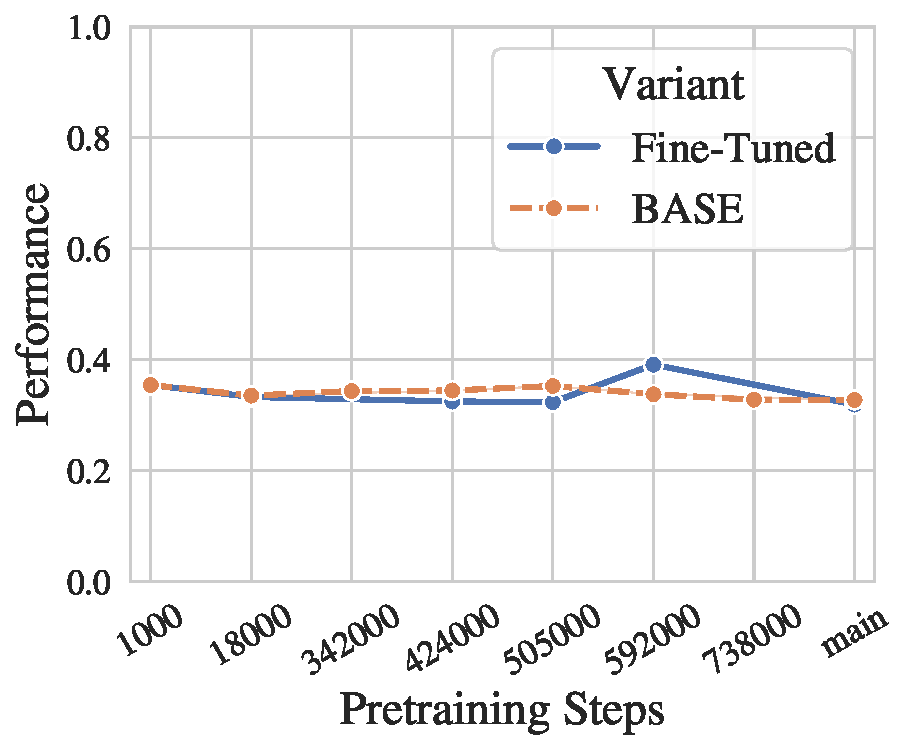
\includegraphics[width=\the\columnwidth]{figures/fig_files/cross-task/sft_evalmnli_matched-trainpaws.pdf}
        \caption{Paws -> MNLI}
    \end{subfigure}%
    ~ 
    \begin{subfigure}[b]{0.3\textwidth}
    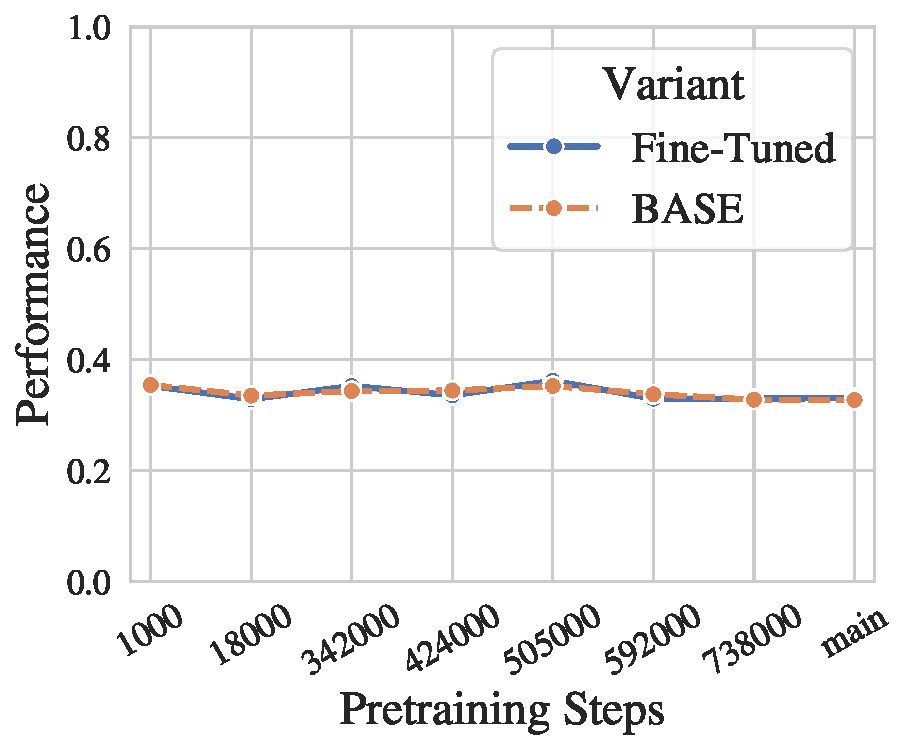
\includegraphics[width=\the\columnwidth]{figures/fig_files/cross-task/sft_evalmnli_matched-trainsocialiqa.pdf}
        \caption{SocialIQA -> MNLI}
    \end{subfigure}%
    ~ 
    \begin{subfigure}[b]{0.3\textwidth}
    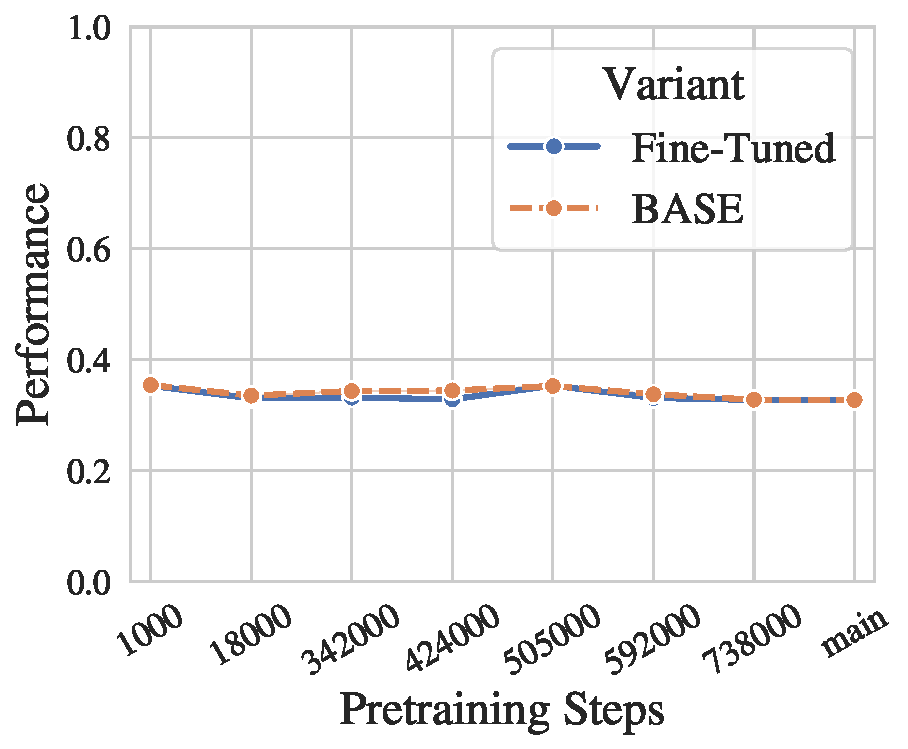
\includegraphics[width=\the\columnwidth]{figures/fig_files/cross-task/sft_evalmnli_matched-trainxsum.pdf}
        \caption{XSum -> MNLI}
    \end{subfigure}%
    \\
    \begin{subfigure}[b]{0.3\textwidth}
    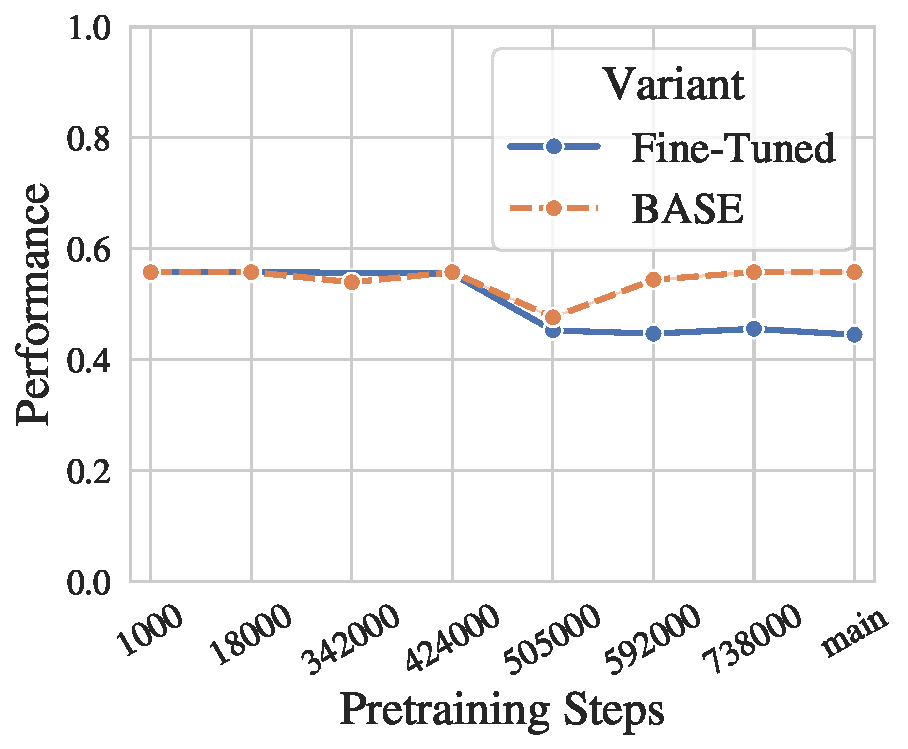
\includegraphics[width=\the\columnwidth]{figures/fig_files/cross-task/sft_evalpaws-trainmnli.pdf}
        \caption{MNLI -> Paws}
    \end{subfigure}%
    ~ 
    \begin{subfigure}[b]{0.3\textwidth}
    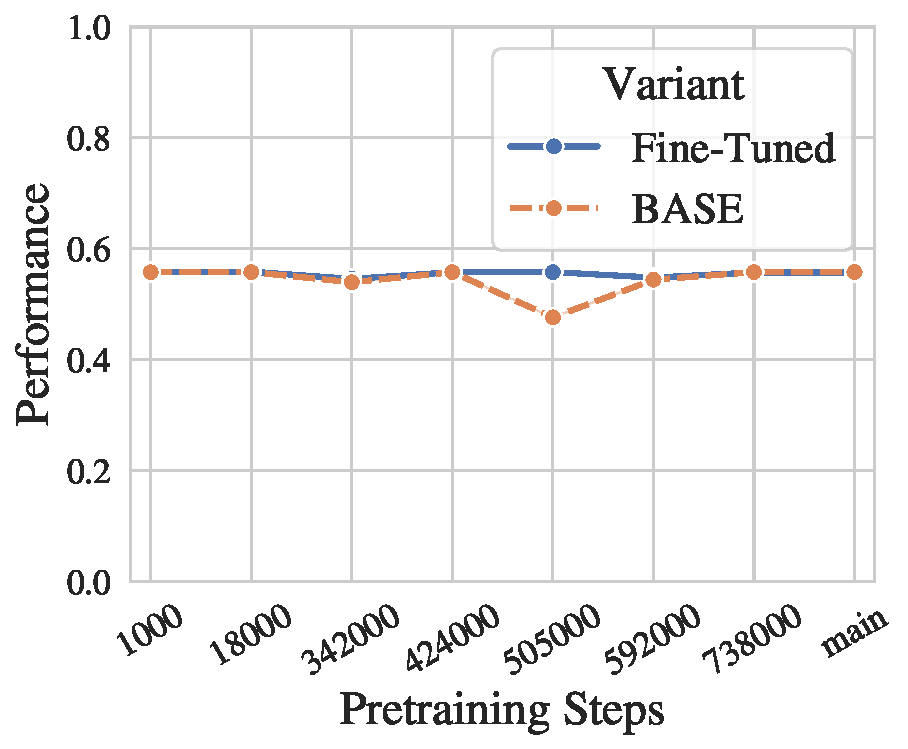
\includegraphics[width=\the\columnwidth]{figures/fig_files/cross-task/sft_evalpaws-trainsocialiqa.pdf}
        \caption{SocialIQA -> Paws}
    \end{subfigure}%
    ~ 
    \begin{subfigure}[b]{0.3\textwidth}
    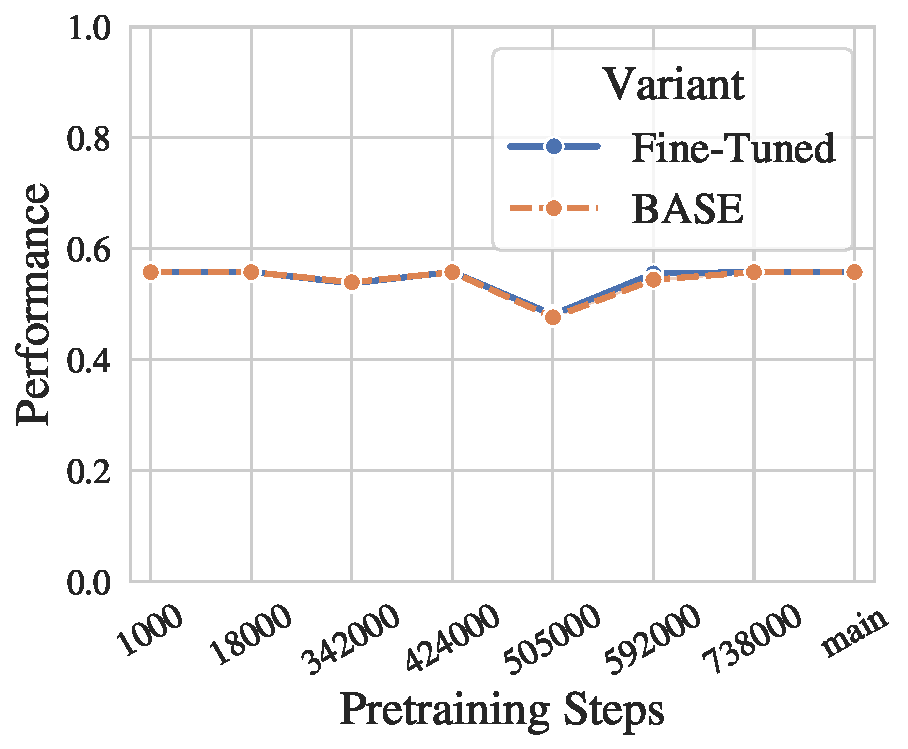
\includegraphics[width=\the\columnwidth]{figures/fig_files/cross-task/sft_evalpaws-trainxsum.pdf}
        \caption{XSum -> Paws}
    \end{subfigure}%
    \\
    \caption{Cross-task performance after supervised fine-tuning on each pre-training step. The model is fine-tuned on a classification task and evaluated on a generation task or a classification task with a different label set.}
    \label{fig:cross-task-ckpt-perf-class}
\end{figure*}

\begin{figure*}[t!]
    \centering
    \begin{subfigure}[b]{0.3\textwidth}
    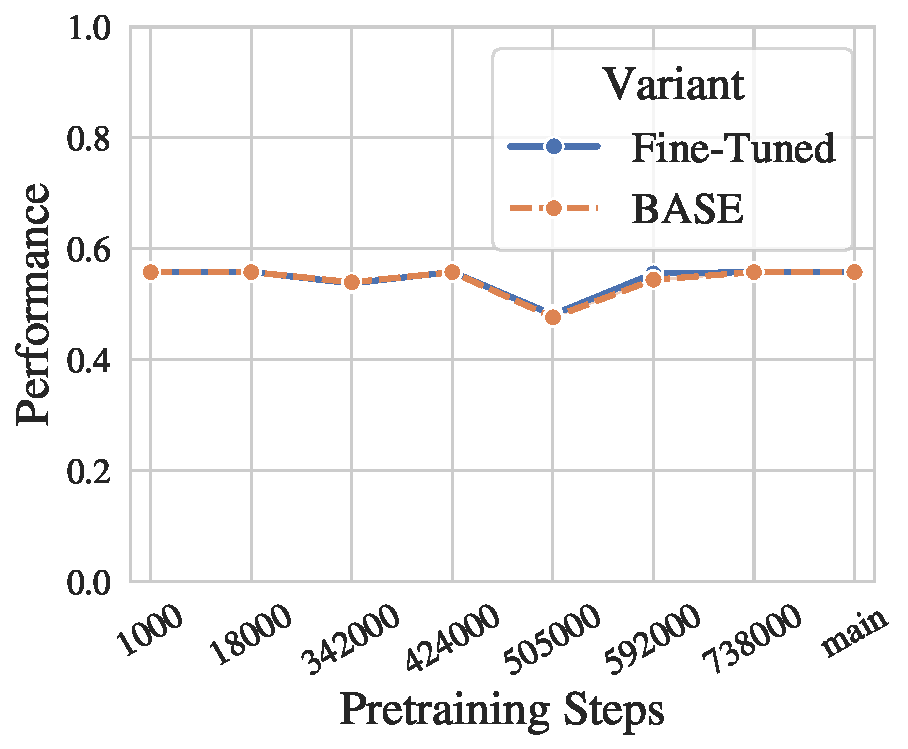
\includegraphics[width=\the\columnwidth]{figures/fig_files/cross-task/sft_evalpaws-trainxsum.pdf}
        \caption{Paws -> XSum}
    \end{subfigure}%
    ~ 
    \begin{subfigure}[b]{0.3\textwidth}
    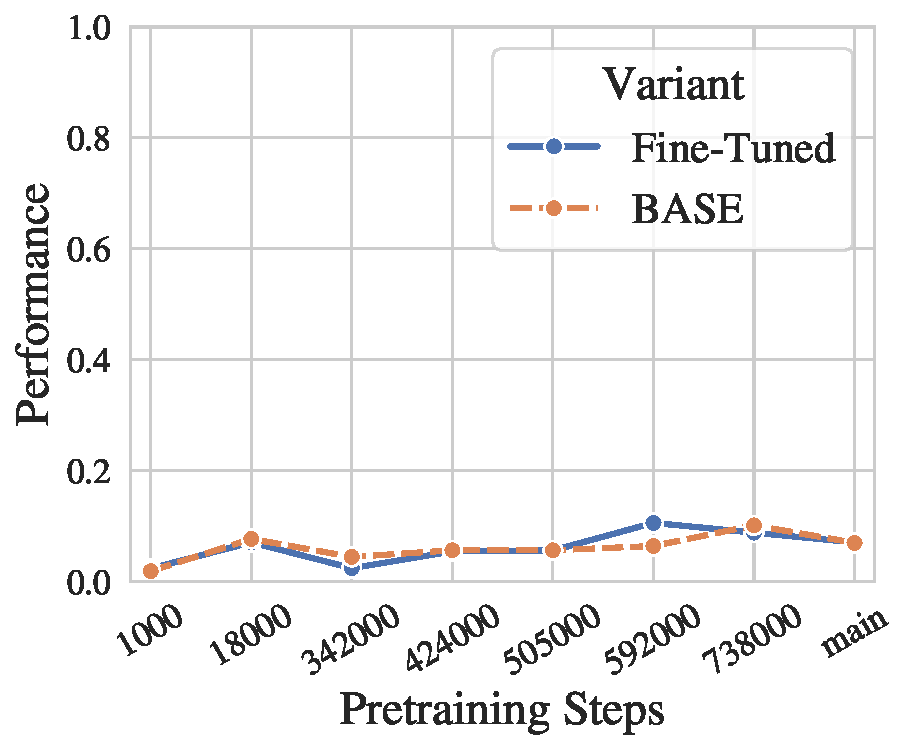
\includegraphics[width=\the\columnwidth]{figures/fig_files/cross-task/sft_evalsocialiqa-trainxsum.pdf}
        \caption{SocialIQA -> XSum}
    \end{subfigure}%
    ~ 
    \begin{subfigure}[b]{0.3\textwidth}
    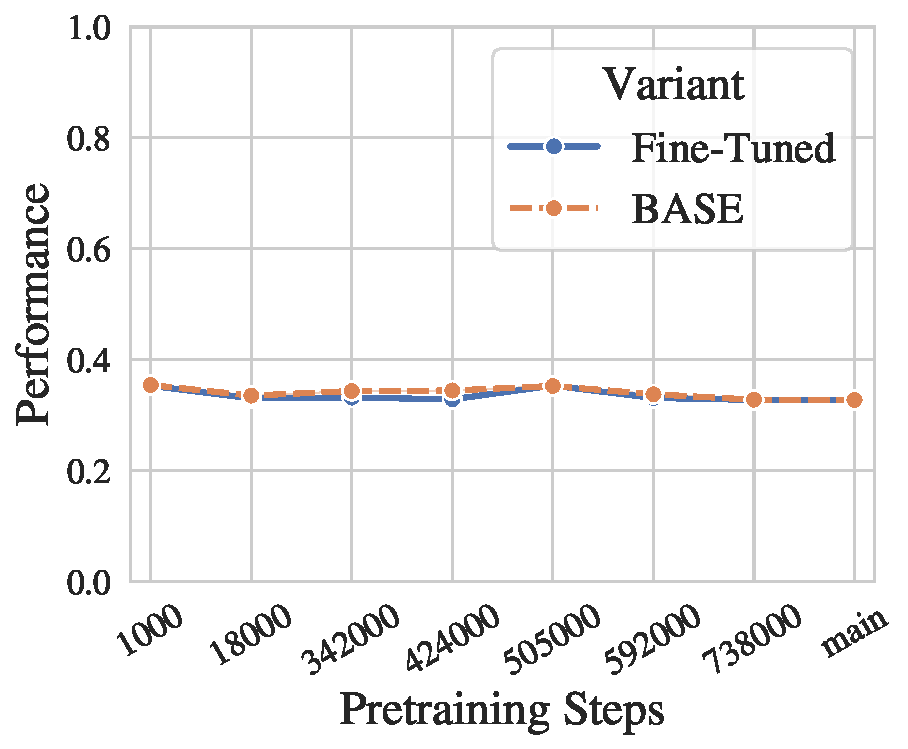
\includegraphics[width=\the\columnwidth]{figures/fig_files/cross-task/sft_evalmnli_matched-trainxsum.pdf}
        \caption{MNLI -> XSum}
    \end{subfigure}%
    \\
    \begin{subfigure}[b]{0.3\textwidth}
    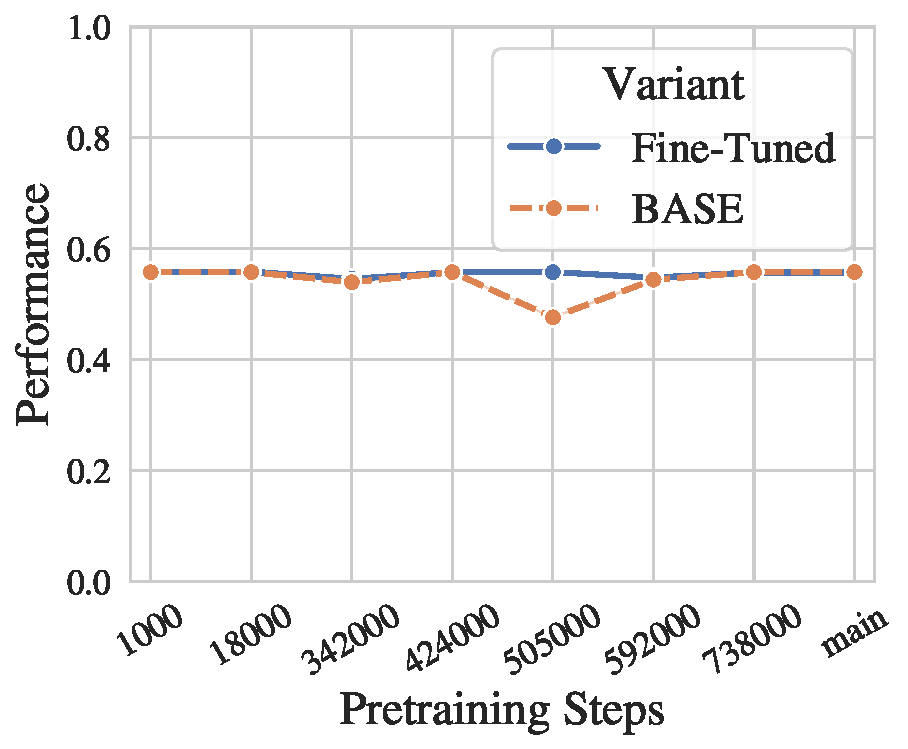
\includegraphics[width=\the\columnwidth]{figures/fig_files/cross-task/sft_evalpaws-trainsocialiqa.pdf}
        \caption{Paws -> SocialIQA}
    \end{subfigure}%
    ~ 
    \begin{subfigure}[b]{0.3\textwidth}
    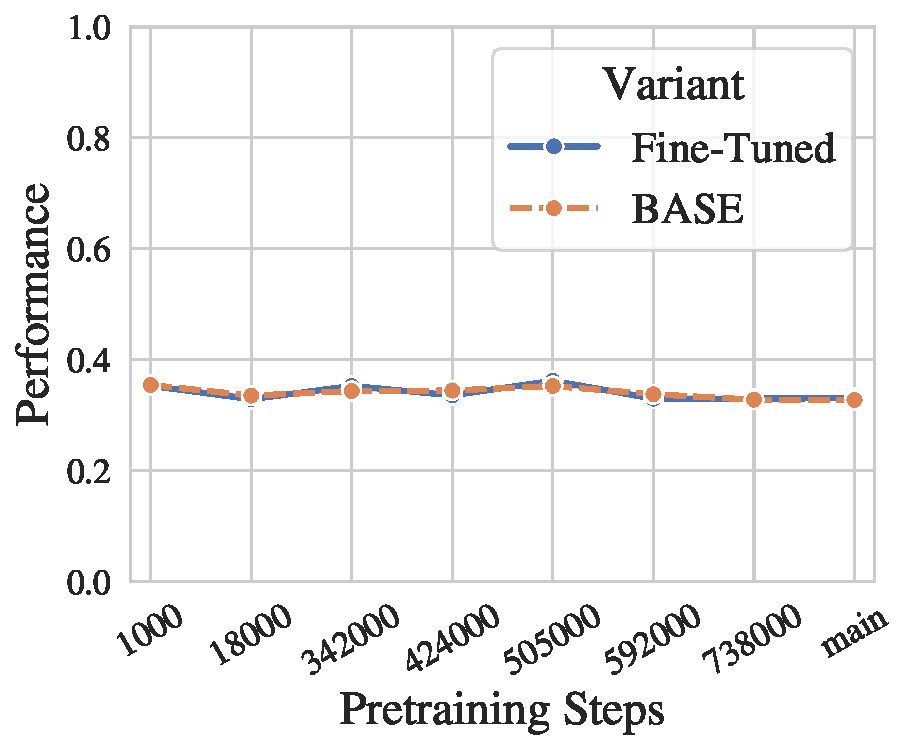
\includegraphics[width=\the\columnwidth]{figures/fig_files/cross-task/sft_evalmnli_matched-trainsocialiqa.pdf}
        \caption{MNLI -> SocialIQA}
    \end{subfigure}%
    ~ 
    \begin{subfigure}[b]{0.3\textwidth}
    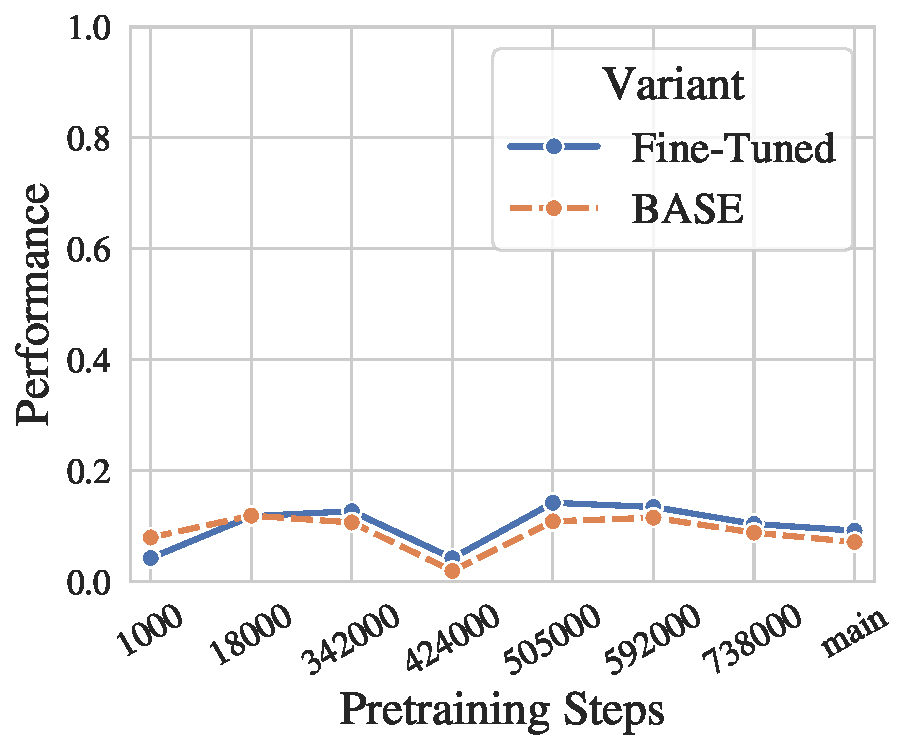
\includegraphics[width=\the\columnwidth]{figures/fig_files/cross-task/sft_evalxsum-trainsocialiqa.pdf}
        \caption{XSum -> SocialIQA}
    \end{subfigure}%
    \\
    \caption{Cross-task performance after supervised fine-tuning on each pre-training step. The model is fine-tuned on a generation task and evaluated on a classification task.}
    \label{fig:cross-task-ckpt-perf-gen}
\end{figure*}